\subsection{Implementation}

Um eine Karte von einem Gebiet $ \Omega \subset \mathbb{R}^2$ zu erstellen, fährt das Auto auf einer Strecke mit konstanter, vorher definierter Geschwindigkeit $v$. Dabei kann das Auto mittels einer implementierten Spurverfolgung autonom oder manuell durch eine externe Lenkung fahren. 
Während der Fahrt werden sowohl die Bilder der Kamera 
als auch die Winkelbeschleunigung um die $z$-Achse 
aufgenommen. Am Ende der Fahrt wird iterativ eine geschätzte Postion des Autos in der Welt zu jedem Zeitpunkt berechnet.

Die Position und Orientierung des Autos lassen sich mit den Weltkoordinaten $x,y$ und einem Winkel $\phi$ beschreiben. Die Startwerte $x(0),y(0)$ und $\phi(0)$ können beliebig gewählt werden. Um nun die nächste Orientierung zu berechnen, wird zu erst die Winkelgeschwindigkeit $\omega$ und die konstante Geschwindigkeit $v$ verwendet.
$$
\begin{aligned}
\phi(i+1)&=\phi(i)+\omega(i)\\
x(i+1)&=x(i)+\cos(\phi(i))\cdot v\\
y(i+1)&=y(i)+\sin(\phi(i))\cdot v
\end{aligned}
$$

\hspace{-12mm}
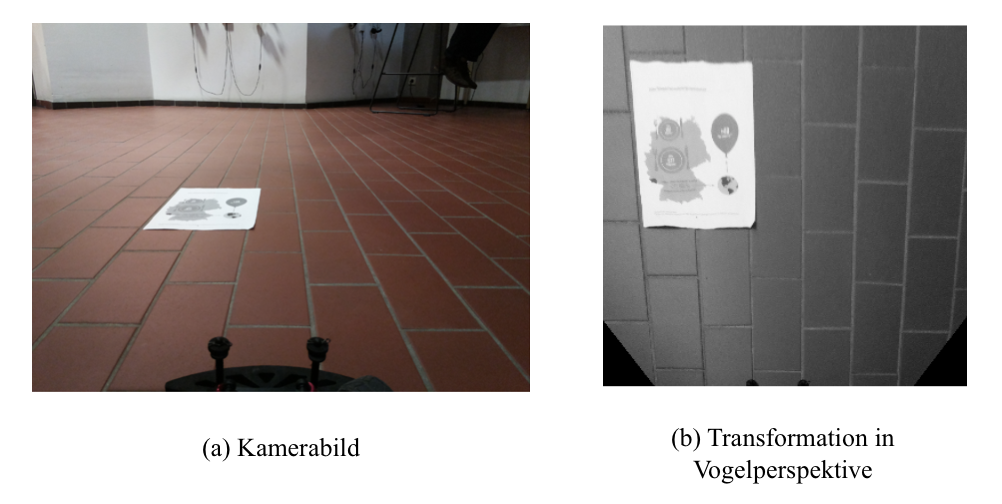
\includegraphics[scale=1]{vogel.png}


Dies ist eine gute erste Schätzung für die tatsächliche Position. Mithilfe der Videodaten soll diese Schätzung nun verbessert werden. Im ersten Schritt wird dazu jedes Bild des Videos in die Vogelperspektive transformiert. Dies hat den Vorteil, dass eine Draufsicht erzeugt wird, in der Abstände in der realen Welt linear vom Pixelabstand abhängen, solange sie in der Ebene liegen. Sei nun 
$\Omega^*_{i}:=\bigcup_{j=1}^i\Omega_i$ das bereits kartografierte Gebiet,
$K_i:\Omega^*_{i} \rightarrow \mathbb{R}$ die Karte, die bis zu Zeitpunkt $i$ erstellt wurde und $V_{i+1}:\Omega_{i+1}\rightarrow \mathbb{R}$ das Bild der Vogelperspektive zum Zeitpunkt $i+1$. Nun soll das Bild $V_{i+1}$ bestmöglich in die Karte $K_i$ integriert werden. Dafür betrachten wir das folgende Variationsproblem mit $(x,y,\phi)\in \Omega \times [-\pi,\pi)$ und der Annahme $|\Omega_{i+1}\cap \Omega^*_i|>\frac{|\Omega_{i+1}|}{2}$:
$$E_{i+1}(x,y,\phi):= \frac{1}{|\Omega_{i+1}\cap \Omega^*_{i}|}\sum_{(u,v) \in \Omega_{i+1}\cap \Omega^*_{i}} |K_{i}(u,v)-V_{i+1}(u+x\cos(\phi),v+y\sin(\phi))|^2 \rightarrow \textnormal{min} $$
Dieses Problem lösen wir nun durch Diskretisierung bei der wir die zuvor geschätzten Werte $x,y$ und $\phi$ als Iterationsstart benutzen können, um schneller zu einer Lösung zu kommen. Hierdurch erhalten wir die Transformationsparameter um das Bild $V_{i+1}$ mit der Karte $K_i$ zu kombinieren, sodass wir die Karte $K_{i+1}$ erhalten. Außerdem lassen sich die zuvor geschätzten Werte aktualisieren.


\hspace{-10mm}
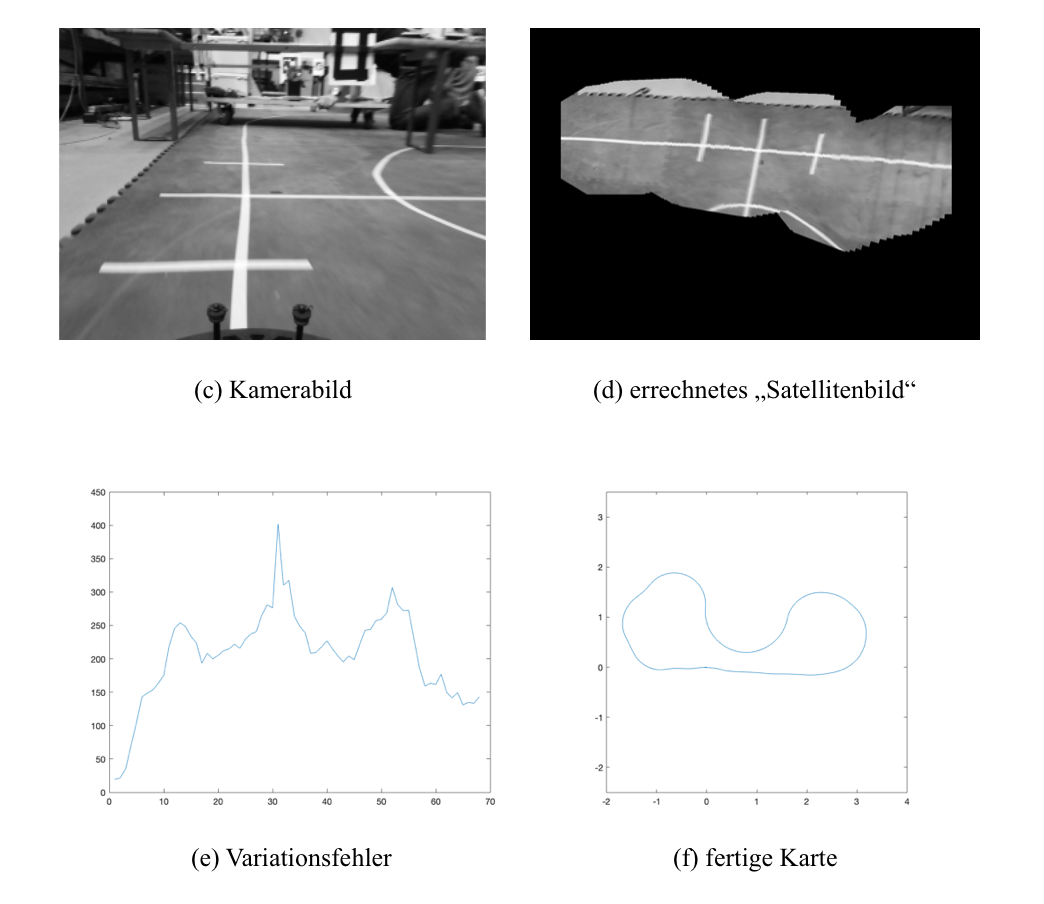
\includegraphics[scale=1]{3456.png}



\subsection{Ausblick}
Für die Zukunft kann eine Fahrt mit gut sichtbaren Makern realisiert werden. Mit den bekannten Markerpositionen kann die vorher bestimmte geschätzte Autoposition verglichen werden. Durch einen solchen Vergleich kann ein zuvor entstandener aufsummierter Fehler minimiert werden. \\
Des Weiteren kann durch einen Plattformwechsel (Python oder Robot Operating System (ROS)) die allgemeine Performace verbessert werden.  So führt eine höhere Kameraauflösung zu einer genaueren Kartenerstellung. Außerdem könnte über eine drahtlose Verbindung zu einem PC eine Karte in Echtzeit generiert werden.   \\
Mit einer verbesserten Kartengenauigkeit kann das Auto nach einer ersten erfolgreich gefahrenen Runde die gesammelten Daten für die eigene Navigation nutzen. Dafür muss die aktuelle geschätzte Position mit der bestehenden Karte abgeglichen und ggf. korrigiert werden.\\

